\section{Nowcasting: mixed frequency Bayesian VAR}
\label{chapter3_section3}


Mixed frequency Bayesian VARs have been proposed recently as an extension to regular Bayesian VAR models. The aim is to account for datasets at mixed frequencies, in the hope of improving nowcasting performances. The reference paper is \cite{Schorfheide2015}, and the developments below follow closely their methodologies. Because mixed frequency Bayesian VAR operate as an augmentation to regular Bayesian VARs, readers unfamiliar with the Bayesian VAR approach are advised to refer first to section \ref{chapter3_section5} where they are covered in details.



\subsection{Formulation}
\label{chapter3_section3_subsection1}


Assume one wants to estimate a VAR with both monthly and quarterly series. There are $m$ monthly series and $q$ quarterly series, implying a total of $n = m + q$ series in the VAR model. At each sample period $t = 1, \cdots, T$, the obervation $y_t$ can thus be separated into its monthly component $y_{m,t}$ and its quarterly component $y_{q,t}$. At quaterly months (months at which quarterly release occur, e.g. March, June, September and December for GDP), $y_{q,t}$ is of dimension $q$ and thus $y_t = \{y_{m,t}, y_{q,t}\}$ is of dimension $n$. The other months, $y_{q,t} = \varnothing$ (there is no release and thus no quarterly data for this month), so that $y_t = \{y_{m,t}\}$ is of dimension $m$ only.

A VAR model requires a panel of series at a single frequency. It is thus assumed further that there exists a series of unobserved monthly components $x_t$ for $t = 1, \cdots, T$ on which the VAR model will be estimated. $x_t$ is an $n$-dimensional vector divided into $x_t = \{x_{m,t}, x_{q,t}\}$, with $x_{m,t}$ an $m$-dimensional component corresponding to the monthly series, and $x_{q,t}$ a $q$-dimensional component corresponding to the partially unobserved quarterly series. Clearly, $x_{m,t} = y_{m,t}$. However, $x_{q,t} \neq y_{q,t}$: the latter is a partial quarterly dataset, while the former represents its full unobserved monthly counterpart.

The VAR model is assumed to exist for the monthly series $x_t$. It is formulated as:

\begin{equation}
x_t = c + A_1 x_{t-1} + \cdots + A_p x_{t-p} + \varepsilon_t \hspace{2cm}
\varepsilon_t \sim N(0, \Sigma)
\label{equation_c3_s3_ss1_1}
\end{equation}

Denote by $x$ the full series $\{x_1, x_2, \cdots, x_T\}$. Also, stack all the VAR coefficients in a single vector $\beta$, as in section \ref{chapter3_section5}. Estimating the model then consists in estimating the unknown parameters $x, \beta$ and $\Sigma$.



\subsection{Estimation}
\label{chapter3_section3_subsection2}


The Bayesian approach consists in obtaining the posterior distributions of $x, \beta$ and $\Sigma$ from a basic application of Bayes rule:

\begin{equation}
\pi(x, \beta, \Sigma| y) \propto f(y|x) \pi(x|\beta, \Sigma) \pi(\beta) \pi(\Sigma)
\label{equation_c3_s3_ss2_1}
\end{equation}

$\pi(x, \beta, \Sigma| y)$ denotes the joint posterior distribution for $x$, $\beta$ and $\Sigma$. $f(y|x)$  is the likelihood function. Because $\beta$ and $\Sigma$ become redundant once $x$ is determined, they can be omitted from the latter which hence writes $f(y|x)$ and not $f(y|x, \beta, \Sigma)$. $\pi(x|\beta, \Sigma)$, $\pi(\beta)$ and $\pi(\Sigma)$ represent the joint prior $\pi(x, \beta, \Sigma)$. Indeed, one can note that:

\begin{equation}
\pi(x, \beta, \Sigma) = \frac{\pi(x, \beta, \Sigma)}{\pi(\beta, \Sigma)} \pi(\beta, \Sigma)
= \pi(x|\beta, \Sigma) \pi(\beta, \Sigma) = \pi(x|\beta, \Sigma) \pi(\beta) \pi(\Sigma)
\label{equation_c3_s3_ss2_2}
\end{equation}

where the final term obtains from the independance assumption between $\beta$ and $\Sigma$. It is worth noting on the other hand that $x$ is not independant from $\beta$ and $\Sigma$. This is clearly implied by equation \ref{equation_c3_s3_ss2_2} and justifies the conditional prior $\pi(x|\beta, \Sigma)$. Such a prior where one parameter of the model is conditional on other model parameters is called a hierarachical prior.

The prior distributions for $\beta$ and $\Sigma$ are similar to those used in section \ref{chapter3_section5} and are thus respectively: $\pi(\beta) \sim N(\beta_0, \Omega_0)$ and $\pi(\Sigma) \sim IW(S_0, \nu_0)$, with respective densities:

\begin{equation}
\pi(\beta) = (2 \pi)^{-nq/2} |\Omega_0|^{-1/2} \exp \left[ -\frac{1}{2} (\beta - \beta_0)' \Omega_0^{-1} (\beta - \beta_0) \right]
\label{equation_c3_s3_ss2_3}
\end{equation}

and:

\begin{equation}
\pi(\Sigma) = (2^{\nu_0 n /2} \Gamma_n(\nu_0/2))^{-1} |S_0|^{\nu_0/2} |\Sigma|^{-(\nu_0+n+1)/2} \exp \left[ - \frac{1}{2} tr \{ \Sigma^{-1} S_0 \}  \right]
\label{equation_c3_s3_ss2_4}
\end{equation} 

For $x$, one notes that conditional on $\beta$ and $\Sigma$, equation \ref{equation_c3_s3_ss1_1} is similar to the VAR model \ref{equation_c3_s5_ss1_1}. Following, the prior for $x$ is also multivariate normal, with density function given by \ref{equation_c3_s5_2}:

\begin{equation}
\pi(x| \beta, \Sigma) = (2 \pi)^{-nT/2} |\bar{\Sigma}|^{-1/2} \exp \left[ -\frac{1}{2} (x-\bar{W} \beta)' \bar{\Sigma}^{-1} (x-\bar{W} \beta) \right]
\label{equation_c3_s3_ss2_5}
\end{equation}

with:

\begin{equation}
x =  vec(X) \hspace{8mm} X = \left( \begin{matrix} x_1' \\ x_2' \\ \vdots \\ x_T' \end{matrix} \right) \hspace{8mm}
\bar{\Sigma} = \Sigma \otimes I_T  \hspace{8mm}
\bar{W} = I_n \otimes W \hspace{8mm}
W = \left( \begin{matrix} 1 & x_0 & \cdots & x_{1-p} \\ 1 & x_1 & \cdots & x_{2-p} \\ \vdots & \vdots & \ddots & \vdots \\ 1 & x_{T-1} & \cdots & x_{T-p} \end{matrix} \right)
\label{equation_c3_s3_ss2_6}
\end{equation}

The joint posterior \ref{equation_c3_s3_ss2_1} is clearly intractable (it cannot be marginalised for $x$, $\beta$ and $\Sigma$ analytically) so the use of the Gibbs sampling algorithm is required. The conditional posteriors for $\beta$ and $\Sigma$ are fairly straightforward. For $\beta$, start from the joint posterior \ref{equation_c3_s3_ss2_1} and relegate to the normalizing constant any term not involving $\beta$. This yields $\pi(\beta| y, x, \Sigma) \propto \pi(x|\beta, \Sigma) \pi(\beta)$. Given \ref{equation_c3_s3_ss2_3} and \ref{equation_c3_s3_ss2_5}, the resulting expression after manipulations is similar to \ref{equation_c3_s5_9}:

\begin{equation}
\pi(\beta| y, x, \Sigma) \propto \exp \left[ -\frac{1}{2} (\beta - \bar{\beta})' \bar{\Omega}^{-1} (\beta - \bar{\beta}) \right]
\label{equation_c3_s3_ss2_7}
\end{equation}

with:

\begin{equation}
\bar{\Omega} = \left( \Omega_0^{-1} + \Sigma^{-1} \otimes W'W \right)^{-1} \hspace{10mm}
\bar{\beta} = \bar{\Omega} \left(\Omega_0^{-1} \beta_0 + (\Sigma^{-1} \otimes W') x \right)
\label{equation_c3_s3_ss2_8}
\end{equation}

\ref{equation_c3_s3_ss2_7} is the kernel of a multivariate normal distribution: $\pi(\beta| y, x, \Sigma) \sim N(\bar{\beta}, \bar{\Omega})$.

Similarly, the conditional posterior $\pi(\Sigma| y, x, \beta)$ obtains from \ref{equation_c3_s3_ss2_1} by relegating to the normalization constant any term not involving $\Sigma$: $\pi(\Sigma|y, x, \beta) \propto \pi(x|\beta, \Sigma) \pi(\Sigma)$. Given \ref{equation_c3_s3_ss2_4} and \ref{equation_c3_s3_ss2_5}, and some manipulations, the result is similar to \ref{equation_c3_s5_12}:

\begin{equation}
\pi(\Sigma| y, x, \beta) \propto |\Sigma|^{(\bar{\nu} + n + 1)/2} \exp \left[ -\frac{1}{2} tr \{ \Sigma^{-1} \bar{S} \} \right]
\label{equation_c3_s3_ss2_9}
\end{equation}

with:

\begin{equation}
\bar{S} = (X - WB)'(X - WB) + S_0 \hspace{10mm} \bar{\nu} = T + \nu_0
\label{equation_c3_s3_ss2_10}
\end{equation}

\ref{equation_c3_s3_ss2_10} is the kernel of an inverse Wishart distribution: $\pi(\Sigma| y, x, \beta) \sim IW(\bar{S}, \bar{\nu})$.

The conditional posterior $\pi(x| y, \beta, \Sigma)$ for $x$ is the most difficult to estimate. Starting from \ref{equation_c3_s3_ss2_1} and relegating to the normalization constant any term not involving $x$ yields $\pi(x| y, \beta, \Sigma) \propto f(y|x) \pi(x|\beta, \Sigma)$. However, the $x_t$ are hidden state variables which makes the formula impossible to apply directly. The solution in this case has been proposed by \cite{Carter1994}. It consists in formulating the conditional posterior $\pi(x| y, \beta, \Sigma)$ in state-space form, then use a Kalman filter procedure to recover the distribution.

To start with, reformulate the dynamic equation \ref{equation_c3_s3_ss1_1} in companion form:

\begin{equation}
\left( \begin{matrix} x_{t} \\ x_{t-1} \\ \vdots \\ x_{t-p+1} \end{matrix} \right) = 
\left( \begin{matrix} c \\ 0 \\ \vdots \\ 0 \end{matrix} \right) +
\left( \begin{matrix} A_{1} & \cdots & A_{p-1} & A_{p} \\ I_n & \cdots & 0 & 0 \\ \vdots & \ddots & \vdots & \vdots \\ 0 & \cdots & I_n & 0 \end{matrix} \right)
\left( \begin{matrix} x_{t-1} \\ x_{t-2} \\ \vdots \\ x_{t-p} \end{matrix} \right) +
\left( \begin{matrix} \varepsilon_t \\ 0 \\ \vdots \\ 0 \end{matrix} \right)
\label{equation_c3_s3_ss2_11}
\end{equation}

More compactly:

\begin{equation}
z_t =  \delta + \Phi \ z_{t-1} + v_t \hspace{20mm} v_t \sim N(0, \Omega)
\label{equation_c3_s3_ss2_12}
\end{equation}

with:

\begin{equation}
z_t = \left( \begin{matrix} x_{t} \\ x_{t-1} \\ \vdots \\ x_{t-p+1} \end{matrix} \right) \hspace{2mm}
\delta = \left( \begin{matrix} c \\ 0 \\ \vdots \\ 0 \end{matrix} \right) \hspace{2mm}
\Phi = \left( \begin{matrix} A_{1} & \cdots & A_{p-1} & A_{p} \\ I_n & \cdots & 0 & 0 \\ \vdots & \ddots & \vdots & \vdots \\ 0 & \cdots & I_n & 0 \end{matrix} \right) \hspace{2mm}
v_t = \left( \begin{matrix} \varepsilon_t \\ 0 \\ \vdots \\ 0 \end{matrix} \right) \hspace{2mm}
\Omega = \left( \begin{matrix} \Sigma & 0 & \cdots & 0 \\ 0 & 0 & \cdots & 0 \\ \vdots & \vdots & \ddots & \vdots \\ 0 & 0 & \cdots & 0 \end{matrix} \right)
\label{equation_c3_s3_ss2_13}
\end{equation}

The simplest way to represent the link between the observed variables $y_t$ and the unobserved components $x_t$ is by the way of selection matrices:

\begin{equation}
y_t = \Lambda_t \ z_t
\label{equation_c3_s3_ss2_14}
\end{equation}

For quarterly months, we have simply the identity $y_t = x_t$. Hence:

\begin{equation}
\Lambda_t = \left( \begin{matrix} I_n \ 0_{n,n(p-1)} \end{matrix} \right)
\label{equation_c3_s3_ss2_15}
\end{equation}

For non-quarterly months, we have $y_t = x_{m,t}$, which results in the definition:

\begin{equation}
\Lambda_t = \left( \begin{matrix} I_m \ 0_{m,q} \ 0_{m,n(p-1)} \end{matrix} \right)
\label{equation_c3_s3_ss2_16}
\end{equation}

\ref{equation_c3_s3_ss2_12} and \ref{equation_c3_s3_ss2_14} represent, respectively, the state equation and observation equation of a state-space system. It is then possible to derive the conditional posterior distribution $\pi(x| y, \beta, \Sigma)$ from the \cite{Carter1994} algorithm. The details of the algorithm can be found in Appendix \ref{appendix3}.

The Gibbs sampling algorithm for the mixed frequency Bayesian VAR then goes as follows:

\textbf{Algorithm 3: Gibbs sampling for the mixed frequency Bayesian VAR} \vspace{3mm} \\
1. Initiate $\beta^{(0)}$, $\Sigma^{(0)}$ and $x^{(0)}$ with any values. In practice, use $x_{m,t} = y_{m,t}$ for the high frequency data, and define $x_{q,t} = y_{q,t}$, with replications of the last observed value for the missing entries. Then set $\beta^{(0)} = \hat{\beta}$ and $\Sigma^{(0)} = \hat{\Sigma}$, where the values are obtained from OLS estimation of \ref{equation_c3_s3_ss1_1} with $x^{(0)}$. Also decide the total number of repetitions of the algorithm (say $r$=2000 for instance), and the number of initial iterations to discard (for instance $d$ = 1000) to ensure convergence.

2. Draw $\beta^{(1)}$ from the conditional distribution $\pi(\beta^{(1)}| y, \Sigma^{(0)}, x^{(0)} ) \sim N(\bar{\beta}, \bar{\Omega})$.

3. Draw $\Sigma^{(1)}$ from the conditional distribution $\pi(\Sigma^{(1)}| y, \beta^{(1)}, x^{(0)}) \sim IW(\bar{S}, \bar{\nu})$.

4. Draw $x^{(1)}$ from the conditional distribution $\pi(x^{(1)}| y, \beta^{(1)}, \Sigma^{(1)})$, using the  Carter-Kohn algorithm.

5. Repeat $r$ times: \\
draw $\beta^{(n)}$ from $\pi(\beta^{(n)}| y, \Sigma^{(n-1)}, x^{(n-1)}) \sim N(\bar{\beta}, \bar{\Omega})$. \\
draw $\Sigma^{(n)}$ from the conditional distribution $\pi(\Sigma^{(n)}| y, \beta^{(n)}, x^{(n-1)}) \sim IW(\bar{S}, \bar{\nu})$. \\
draw $x^{(n)}$ from $\pi(x^{(n)}| y, \beta^{(n)}, \Sigma^{(n)})$, using the Carter-Kohn algorithm.

6. Discard $d$ initial observations as burn-in sample to make sure convergence is achieved. Then the remaining values are draws from the unconditional posteriors $\pi(\beta| y)$, $\pi(\Sigma| y)$ and $\pi(x| y)$, which can be used to recover an empirical distribution.

\newpage

\subsection{Prediction}
\label{chapter3_section3_subsection3}


The MCMC algorithm for predictions is similar to that described in section \ref{chapter3_section5}:

\textbf{Algorithm 4: prediction for the mixed frequency Bayesian VAR} \vspace{3mm} \\
2. draw a value $\beta$ from $\pi(\beta, \Sigma, x|y)$. Recycle a draw from the Gibbs sampling algorithm.

3. draw a value $\Sigma$ from $\pi(\beta, \Sigma, x|y)$. Recycle a draw from the Gibbs sampling algorithm.

1. draw a value $x$ from $\pi(\beta, \Sigma, x|y)$. Recycle a draw from the Gibbs sampling algorithm.

4. conditional on $\beta$, $\Sigma$, and $x$, compute recursively $x_{t+1}, \cdots, x_{t+h}$ from \ref{equation_c3_s3_ss1_1}.

5. convert $x_{t+1}, \cdots, x_{t+h}$ into $z_{t+1}, \cdots, z_{t+h}$.

6. compute $y_{t+1}, \cdots, y_{t+h}$ from $z_{t+1}, \cdots, z_{t+h}$, using \ref{equation_c3_s3_ss2_14}.

7. discard $x$, $\beta$ and $\Sigma$.

8. repeat the process $r-d$ times to obtain $r-d$ draws from the posterior predictive distribution.



\subsection{Application}
\label{chapter3_section3_subsection4}

As a short application, it is interesting to visualize the actual, quarterly series of GDP growth along with the monthly estimates provided by the model. Figure \ref{fig_c3_s3_ss4_1} provides an overview of the results.

\newpage

\begin{figure} [H]
\centering
\begin{subfigure}[t]{0.7\textwidth}
\centering
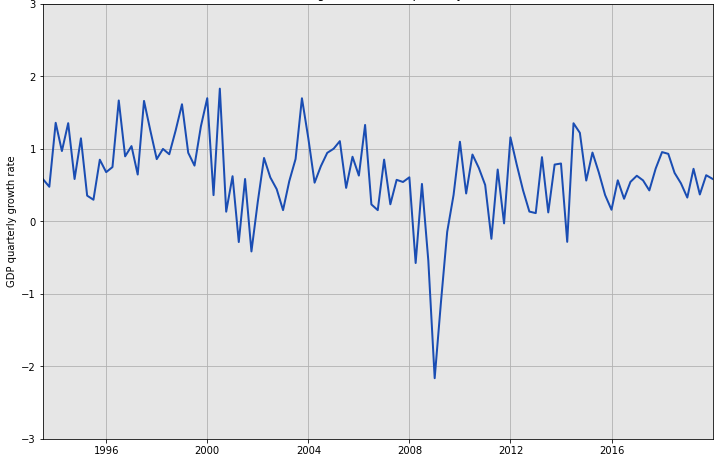
\includegraphics[width=\linewidth]{images/quarterly_gdp.png}
\caption{Actual quarterly values}
\end{subfigure} 	\hspace{1cm} \\
\begin{subfigure}[t]{0.7\textwidth}
\centering
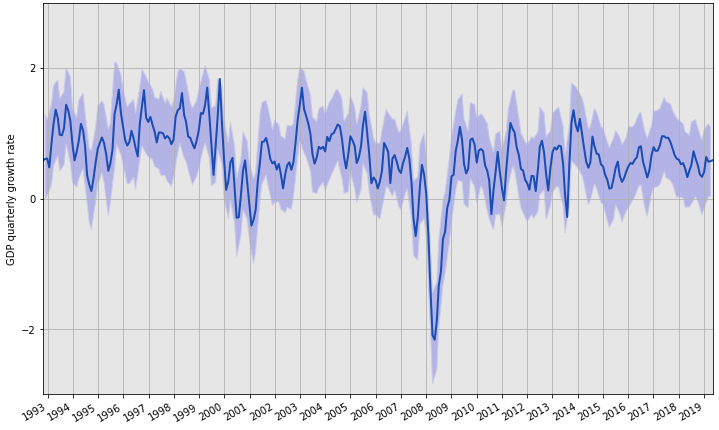
\includegraphics[width=\linewidth]{images/monthly_gdp.png}
\caption{Monthly estimates with 95\% credibility bands}
\end{subfigure}
\caption{Actual values and monthly estimates for GDP growth}
\label{fig_c3_s3_ss4_1}
\vspace{-3mm}
\end{figure}

One can see that the monthly series look quite accurate. This is demonstrated by the tight credibility bands around the median of the posterior. Comparing the two series, they appear to be quite similar. Looking closely at the monthly series however, it looks a bit more jagged than the quarterly series, showing the short term monthly deviations from the quarterly trend. Overall, this graphic reflects well on the ability of the model to infer missing values from the information provided by the rest of the dataset.

\newpage